\clearpage
\section*{Centering ECal without raising the assembly}
Keep TS, tracker, LYSO and all HCal groups at their \emph{original heights}.
Move only ECal by $\Delta X=+46.56$ mm and $\Delta Y=-46.08$ mm, using the same
active-envelope alignment as on the previous page. ECal height, rotations and
internal layer offsets stay unchanged. All 26 active layers are still required.

\textbf{Centering alone gives 2.163 muons/hour without a roof and 1.842 with
3 ft of concrete.} This is a 53.7\% increase over the original layout, and
11.0\% above the raised-and-centred configuration. In this geometry,
raising the assembly is not needed to obtain the gain from ECal alignment.

\subsection*{Removing ECal}
The second test physically removes the entire ECal subtree, including its
passive materials, while keeping every other subsystem at its original position.
The coincidence now requires \textbf{22 active layers}: six TS, four tracker,
two LYSO and ten HCal. It no longer tests passage through an ECal.

\begin{center}
\begin{tabular}{lrrrr}
\toprule
Configuration & Layers & No roof/hour & Concrete/hour & No roof/day\\
\midrule
Original & 26 & 1.407 & 1.199 & 33.8\\
ECal centred only & 26 & 2.163 & 1.842 & 51.9\\
ECal removed & 22 & 2.214 & 1.883 & 53.1\\
\bottomrule
\end{tabular}
\end{center}
Here ``concrete'' means the same 3 ft uniform overhead slab. The 22-layer
geometric reference is $1.5730\pm0.0002$ muons/hour for $p>1$ GeV/$c$;
centering ECal retains 98.5\% of that geometrical coincidence rate while
still requiring all four ECal layers.

\begin{center}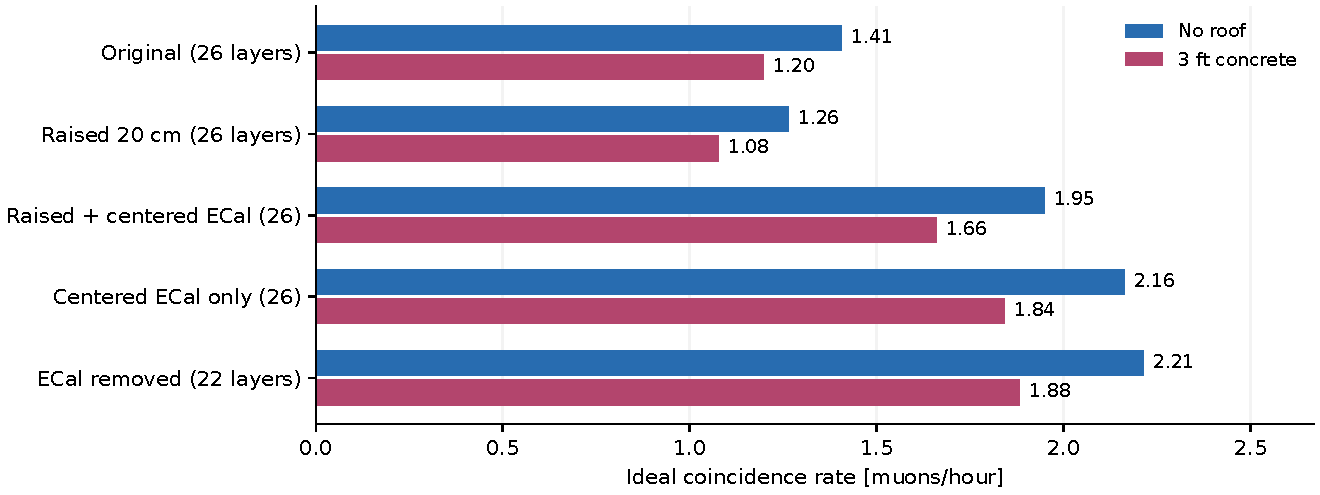
\includegraphics[width=\linewidth]{ecal_comparison/all_layout_rates.pdf}\end{center}
\textbf{Figure 4.} All five configurations under the same incident-spectrum
model. The last row uses the relaxed 22-layer requirement and excludes ECal
material. The raised rows move TS, tracker and LYSO upward by 200 mm;
the two new cases use their original positions.

\textbf{Material treatment.} The centred-only case retains the original
$32.70\ \mathrm{g\,cm^{-2}}$ stopping proxy, consistent with the earlier placement
studies. For ECal removal, ROOT chords for 96 accepted rays give
$24.32\ \mathrm{g\,cm^{-2}}$ for the remaining detector. The same polystyrene
CSDA approximation represents that reduced column. At the original column,
the 22-layer angular acceptance alone would give 2.195 and 1.869
muons/hour; removing ECal material raises them to the values in the table.

\textbf{Checks and limits.} Eight Sobol scrambles of $2^{18}$ trials were run
for each new case, with independent pseudorandom checks. ROOT agrees with all
4,992 layer decisions for centering and all 4,224 for removal in 192-ray tests.
Scattering, straggling, decay, detector inefficiency and mechanical-fit validation
remain outside this estimate. The scripts and results are in
\texttt{ecal\_comparison/}; \texttt{build\_report.sh} rebuilds these sections too.
